% ============================================================
% CSE 8803 IUQ --- Final Report
% Bo Feng (bfeng66@gatech.edu)
% Due: April 27, 2026
% ============================================================

\documentclass[11pt]{article}

% --- Page layout ---
\usepackage[margin=1in]{geometry}
\usepackage{setspace}
\singlespacing

% --- Math ---
\usepackage{amsmath, amssymb, amsthm}
\usepackage{bm}

% --- Fonts & encoding ---
\usepackage[T1]{fontenc}
\usepackage[utf8]{inputenc}
\usepackage{microtype}

% --- Figures & tables ---
\usepackage{graphicx}
\usepackage{booktabs}
\usepackage{multirow}

% --- Hyperlinks ---
\usepackage[colorlinks=true, linkcolor=blue, citecolor=blue, urlcolor=blue]{hyperref}

% --- Bibliography ---
\usepackage{natbib}
\bibliographystyle{plainnat}

% --- Header ---
\usepackage{fancyhdr}
\pagestyle{fancy}
\fancyhf{}
\rhead{\small CSE 8803 IUQ --- Final Report}
\lhead{\small Bo Feng}
\cfoot{\thepage}

% --- Custom commands ---
\newcommand{\bsy}{\bm{y}}
\newcommand{\bstheta}{\bm{\theta}}
\newcommand{\Beta}{\mathrm{Beta}}

\begin{document}

% --- Title block ---
\begin{center}
  {\Large\bfseries LLM-Informed Bayesian Priors for Reducing\\
  Experimental Cost in Behavioral Economics}

  \vspace{0.6em}
  {\normalsize Final Report --- CSE 8803 IUQ, Spring 2026}

  \vspace{0.4em}
  {\normalsize Bo Feng \quad \texttt{bfeng66@gatech.edu}}

  \vspace{0.3em}
  {\small Georgia Institute of Technology \quad April 27, 2026}

  \vspace{0.6em}
  {\small \textbf{Code:} \url{https://github.gatech.edu/bfeng66/cse8803-iuq-project}}

  \vspace{0.2em}
  {\small \textbf{Video:} \url{https://mediaspace.gatech.edu/channel/Spring+2026+CSE+8803+IUQ}\footnote{Channel URL; the direct video URL will replace this placeholder after upload to MediaSpace on Apr 27.}}
\end{center}

\vspace{0.3em}
\hrule
\vspace{0.6em}

% ============================================================
\begin{abstract}
\noindent
Behavioral economic experiments are expensive: each datum costs participant fees, lab time,
and IRB overhead. We ask whether large language model (LLM) simulations can serve as an
informative Bayesian prior, reducing the human sample size needed to reach a target posterior
precision. We model dictator-game sharing ratios with a Beta likelihood and compare two pipelines:
(i) a flat-prior baseline solved by Metropolis--Hastings MCMC, and (ii) a frontier method that
encodes 500 GPT-4o pseudo-observations as a power prior~\citep{ibrahim2000power} and solves the
posterior with Stein Variational Gradient Descent~\citep{liu2016stein}.
On 137 dictator observations from \citet{vonblanckenburg2023giving}, the LLM prior achieves a
sample-size reduction ratio $\rho = n^*_{\mathrm{LLM}}/n^*_{\mathrm{flat}} \approx 0.26$ on the
giving game and $\rho \approx 0.55$ on the taking-game variant; coverage of
95\% posterior-predictive intervals tracks nominal under all but moderate upward prior
misspecification, where it falls to $\sim$83\%. A leakage ablation with \texttt{gpt-3.5-turbo}
(pre-Horton2023 cutoff) recovers an identical $\rho = 0.26$ but with markedly worse coverage
(0.83 vs 0.98 at $n{=}50$), indicating that the gpt-4o advantage is calibration quality, not
sample-size benefit, and that the result is not a pure training-data leakage artefact. We report the compute--accuracy
trade-off, document the regimes where the LLM prior helps and hurts, and discuss when SVGD
becomes a useful inference engine for higher-dimensional extensions of this template.
\end{abstract}

% ============================================================
\section{Introduction}
% ============================================================

Bayesian inference of human behavioral parameters is data-hungry. Eliciting tight posteriors
on traits like generosity or risk aversion routinely requires hundreds of subjects per
condition, at high marginal cost per observation. Yet a contemporary LLM, prompted with the
same instructions an experimenter would read to a participant, can produce thousands of
synthetic decisions in minutes~\citep{horton2023large, argyle2023silicon, aher2023using}.
These ``silicon subjects'' are not human substitutes, but their distribution carries
information about the behavior we are trying to estimate. The relevant question for
uncertainty quantification (UQ) is: \emph{how much real data does an LLM prior save, and
under what conditions does it harm calibration?}

\paragraph{Contribution.}
We instantiate a small but complete LLM-informed Bayesian pipeline on individual-level
dictator-game data~\citep{vonblanckenburg2023giving}, with the following ingredients:
(1) a Beta likelihood on continuous sharing ratios; (2) a baseline flat prior solved by
log-space Metropolis--Hastings (MH); (3) a frontier method with an LLM power prior solved
by Stein Variational Gradient Descent (SVGD); (4) calibration via held-out coverage of 95\%
posterior-predictive intervals; and (5) a sample-size reduction ratio
$\rho = n^*_{\mathrm{LLM}}/n^*_{\mathrm{flat}}$ that quantifies the experimental savings.
On top of this baseline, we conduct four diagnostic studies that the project check-in did
not address: a cross-game replication on the taking-game variant, a continuous misspecification
curve over $\delta \in [-3, +3]$ prior std-deviations, a training-data leakage ablation against
\texttt{gpt-3.5-turbo}, and a compute--accuracy Pareto analysis comparing wall-clock time
and effective sample size of the two inference engines. The combination yields a
fail-mode-aware accounting of when the LLM prior is worth using.

% ============================================================
\section{Related Work}
% ============================================================

\paragraph{LLMs as economic agents.}
\citet{horton2023large} introduces ``homo silicus'' as an LLM-driven simulation tool for
economic experiments, replicating qualitative effects of classic studies. \citet{argyle2023silicon}
and \citet{aher2023using} extend this to political and psychometric tasks. Recent
working papers~\citep{gao2026measure, ludwig2025econometrics} formalize how to weight and
combine LLM evidence with human data; the present work uses the power-prior
construction~\citep{ibrahim2000power} as a transparent, single-knob instantiation of that idea.

\paragraph{Variational inference for posterior approximation.}
SVGD~\citep{liu2016stein} approximates a posterior by a deterministic interacting particle
system whose update direction is the kernelised score of the target. It scales to
intermediate dimensions where MCMC mixing degrades but standard mean-field VI cannot capture
posterior dependence. Our pipeline uses SVGD to instantiate the design pattern; we
report below that for the two-parameter Beta posterior MCMC is faster per equivalent ESS,
and discuss when SVGD becomes attractive as the model dimension grows.

% ============================================================
\section{Method}
% ============================================================

\subsection{Likelihood and quantity of interest}

For each dictator-game observation $y_i \in (0,1)$ (a sharing ratio), we adopt
$y_i \mid \alpha,\beta \sim \Beta(\alpha,\beta)$ independently. With $n$ human observations
$\bsy = (y_1, \ldots, y_n)$ and prior $p(\alpha, \beta)$,
\begin{equation}
  p(\alpha, \beta \mid \bsy) \;\propto\;
  \frac{1}{B(\alpha,\beta)^n}\prod_{i=1}^n y_i^{\alpha-1}(1-y_i)^{\beta-1}
  \cdot p(\alpha, \beta).
  \label{eq:posterior}
\end{equation}
Our primary scalar is the population mean sharing ratio $\mu = \alpha/(\alpha+\beta)$.
The decision-relevant quantity is the \emph{sample-size reduction ratio}
$\rho = n^*_{\mathrm{LLM}}/n^*_{\mathrm{flat}}$, where $n^*$ is the smallest $n$ that
brings $\mathrm{Var}(\mu \mid \bsy_{1:n})$ below a fixed target precision. We choose the
target as the midpoint between the flat-prior posterior variances at the smallest and
largest $n$ in our sweep, so that $\rho$ is well-defined and comparable across runs.

\paragraph{Sources of uncertainty.}
Four sources contribute, and the pipeline must account for each separately.
(a) \emph{Parameter uncertainty} in $(\alpha, \beta)$ -- the inferential target, captured by the
posterior in \eqref{eq:posterior}.
(b) \emph{Observation noise} -- the irreducible Beta sampling spread of an individual
$y_i$ around the population mean, which dominates the posterior-predictive interval at
large $n$ even when parameter uncertainty is small.
(c) \emph{Model error} -- the Beta family is the simplest parametric form for $(0,1)$-valued
data and may mis-fit multi-modal sharing distributions; we treat this as un-modeled and
read it through coverage diagnostics.
(d) \emph{Prior input uncertainty} -- the LLM persona that produces our pseudo-observations
is itself stochastic across model versions, prompts, and temperature, and may drift from the
human population in ways our experiment does not directly observe; the dense
misspecification grid (\S\ref{sec:dense}) and cross-model leakage ablation
(\S\ref{sec:leakage}) probe this source.

\subsection{Baseline: flat prior with log-space Metropolis--Hastings}

We use $p(\alpha,\beta) \propto 1$ on $(0, 100)^2$ as an effectively flat prior. Both
parameters are positive; we sample in $\bm{\eta} = (\log\alpha, \log\beta)$ with isotropic
Gaussian proposals $\bm{\eta}' = \bm{\eta} + \bm{\epsilon}$, $\bm{\epsilon} \sim \mathcal{N}(\bm{0}, 0.3^2 I)$,
and accept with the Hastings ratio
\begin{equation}
  r = \min\!\left(1, \,
  \frac{\pi(\bm{\eta}') \, J(\bm{\eta}')}
       {\pi(\bm{\eta}) \, J(\bm{\eta})}\right),
  \qquad J(\bm{\eta}) = \alpha \beta = e^{\eta_\alpha + \eta_\beta},
  \label{eq:mh}
\end{equation}
i.e.\ multiplying by the log-transform Jacobian. We run 15{,}000 post-burn-in samples
after a 3{,}000-step burn-in.

\subsection{Frontier: LLM power prior with SVGD}

We elicit $M=500$ pseudo-observations $\tilde{y}_1, \ldots, \tilde{y}_M$ from GPT-4o
(temperature $1.0$, ten batches of 50, seed $42+\text{batch}$) using the dictator-game
prompt verbatim from the human protocol. Following \citet{ibrahim2000power}, we encode
this LLM evidence as a \emph{power prior}
\begin{equation}
  p_{\mathrm{LLM}}(\alpha, \beta) \;\propto\; \prod_{j=1}^{M} \Beta(\tilde{y}_j; \alpha, \beta)^{w/M},
  \label{eq:powerprior}
\end{equation}
with effective weight $w$ controlling how many real observations the LLM is worth in
posterior-information units. We use $w=20$ throughout (sensitivity analysis below);
this is roughly one-quarter of the held-out sample, large enough to matter but small enough
not to drown the data.

For inference we run SVGD~\citep{liu2016stein} with $K = 100$ particles
$\{\bm{\eta}^{(k)}\}_{k=1}^K$ in log-space, RBF kernel
$\kappa(\bm{\eta}, \bm{\eta}') = \exp\!\left(-\|\bm{\eta} - \bm{\eta}'\|^2/(2h)\right)$ with
median-heuristic bandwidth, Adam step size $0.05$, and $T = 2{,}000$ iterations. Each
particle is updated by
\begin{equation}
  \bm{\eta}^{(k)}_{t+1} \;=\; \bm{\eta}^{(k)}_t \;+\; \frac{\epsilon_t}{K}\sum_{\ell=1}^{K}
  \!\left[\kappa(\bm{\eta}^{(\ell)}_t, \bm{\eta}^{(k)}_t)\, \nabla_{\bm{\eta}} \log p(\bm{\eta}^{(\ell)}_t \mid \bsy)
  + \nabla_{\bm{\eta}^{(\ell)}_t} \kappa(\bm{\eta}^{(\ell)}_t, \bm{\eta}^{(k)}_t)\right].
  \label{eq:svgd}
\end{equation}
Particles are initialized at the method-of-moments estimate of $(\log\alpha, \log\beta)$
plus Gaussian jitter; gradients are computed analytically via $\psi(\cdot)$ derivatives of
$\log B(\alpha,\beta)$, and clipped to $[-100, 100]$ for stability.

\subsection{Calibration and diagnostics}

We measure \emph{empirical coverage}: for held-out observation $y$, we compute the
posterior-predictive CDF $F(y) = \mathbb{E}_{(\alpha,\beta) \sim p(\cdot\mid\bsy)}\,F_{\Beta}(y; \alpha,\beta)$
using posterior samples and ask whether $F(y) \in [0.025, 0.975]$. Averaging over the held-out
test set gives the empirical coverage of the nominal-95\% interval.
For MCMC we compute effective sample size for $\mu$ via the initial-positive-sequence
estimator~\citep{geyer1992practical}; for SVGD we use the number of particles as a
construction-by-design ESS, while reporting wall-clock time.

% ============================================================
\section{Experiments}
% ============================================================

\subsection{Setup}

Data: 137 individual-level dictator decisions from \citet{vonblanckenburg2023giving},
split as 69 \emph{giving}-game and 68 \emph{taking}-game observations. We held out 30\%
(41 obs) for calibration and used the remaining 96 for inference. All sharing ratios are
clipped to $[10^{-3}, 1-10^{-3}]$ to keep the Beta likelihood finite. All experiments use
seed $42$; LLM elicitation seeds are $42+\text{batch index}$ per API call.

\subsection{Sample-size reduction $\rho$ on the giving game (replication)}

Table~\ref{tab:gp_giving} reports posterior variances of $\mu$ across $n \in \{5,10,20,50,90\}$
under flat and LLM priors with the gpt-4o pseudo-observations. The LLM prior reduces variance
by a factor of $1.27\times$ to $2.62\times$ depending on $n$, with the largest gains at small
$n$ (where the prior carries the most weight in posterior information). Setting the precision
target as the midpoint of the flat-prior endpoints yields
$n^*_{\mathrm{flat}} \approx 19.2$ and $n^*_{\mathrm{LLM}} \approx 5.0$, i.e.\
$\rho \approx 0.26$ -- the LLM prior recovers the same precision with a $74\%$
smaller human sample. Figure~\ref{fig:nstar_giving} plots the variance--$n$ curves on log-log axes.

\begin{table}[h]
  \centering
  \small
  \begin{tabular}{rcccc}
    \toprule
    $n$ & $\mathrm{Var}(\mu)_{\mathrm{flat}} \times 10^3$ & $\mathrm{Var}(\mu)_{\mathrm{LLM}} \times 10^3$
        & Ratio & Coverage 95\% (LLM) \\
    \midrule
    5   & 5.16 & 2.17 & 2.38$\times$ & 0.98 \\
    10  & 4.81 & 1.84 & 2.62$\times$ & 0.98 \\
    20  & 2.88 & 1.41 & 2.04$\times$ & 0.98 \\
    50  & 1.15 & 0.81 & 1.42$\times$ & 0.98 \\
    90  & 0.77 & 0.61 & 1.27$\times$ & 0.98 \\
    \bottomrule
  \end{tabular}
  \caption{Giving game (gpt-4o LLM prior): variance reduction across sample sizes. The LLM
  prior helps most at small $n$; coverage tracks nominal at every $n$.}
  \label{tab:gp_giving}
\end{table}

\begin{figure}[h]
  \centering
  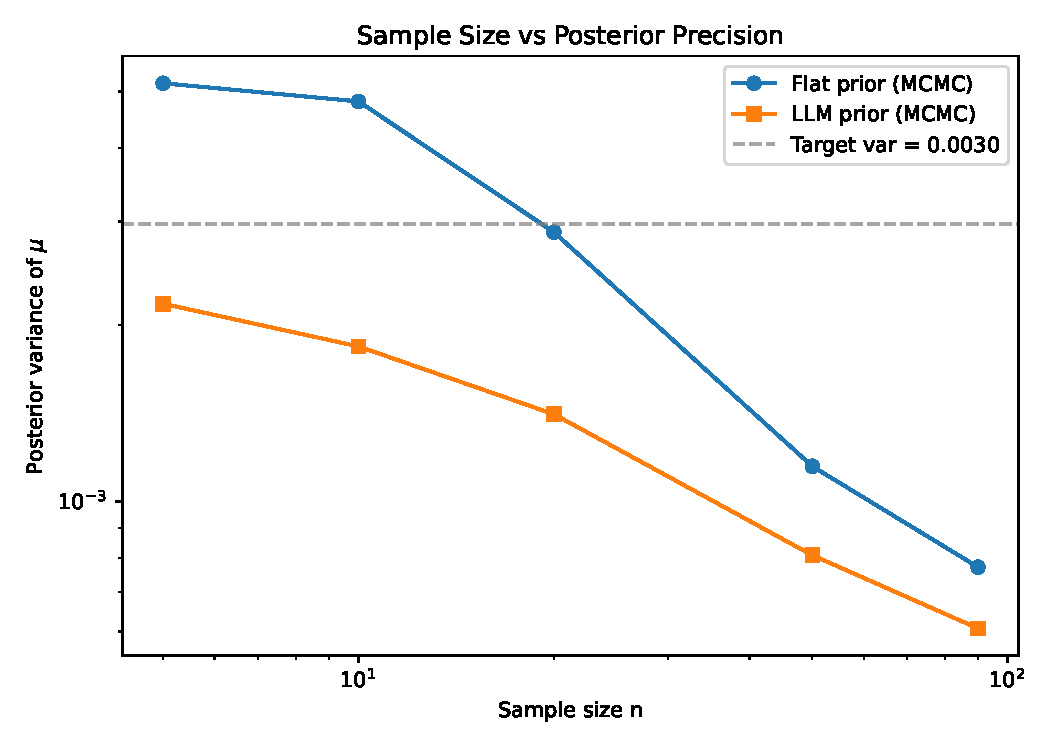
\includegraphics[width=0.55\textwidth]{../figures/nstar_curve.pdf}
  \caption{Posterior variance of $\mu$ vs sample size $n$, giving game. The LLM prior crosses
  the precision target near $n \approx 5$; the flat prior requires $n \approx 19$.}
  \label{fig:nstar_giving}
\end{figure}

\subsection{Cross-game replication (taking-game)}
\label{sec:taking}

The check-in identified cross-game consistency of $\rho$ as the strongest generalization
claim accessible from this dataset. We re-elicited 500 pseudo-observations from GPT-4o under the
taking-game prompt (the agent may take up to \texteuro{}10 from a counterpart's endowment;
we record sharing ratio = $1 - \text{taken}/10$), then ran the full pipeline on the 68
taking-game observations. Table~\ref{tab:gp_taking} and Figure~\ref{fig:nstar_taking}
report the result.

\begin{table}[h]
  \centering
  \small
  \begin{tabular}{rccc}
    \toprule
    $n$ & $\mathrm{Var}(\mu)_{\mathrm{flat}} \times 10^3$
        & $\mathrm{Var}(\mu)_{\mathrm{LLM}} \times 10^3$ & Ratio \\
    \midrule
    5   & 9.73 & 3.24 & 3.00$\times$ \\
    10  & 5.16 & 2.83 & 1.82$\times$ \\
    20  & 2.89 & 2.11 & 1.37$\times$ \\
    35  & 1.86 & 1.36 & 1.36$\times$ \\
    45  & 1.48 & 1.21 & 1.22$\times$ \\
    \bottomrule
  \end{tabular}
  \caption{Taking game: variance reduction across sample sizes (gpt-4o LLM prior); $n^*_{\mathrm{flat}} \approx 9.1$, $n^*_{\mathrm{LLM}} \approx 5.0$, $\rho \approx 0.55$.}
  \label{tab:gp_taking}
\end{table}

\begin{figure}[h]
  \centering
  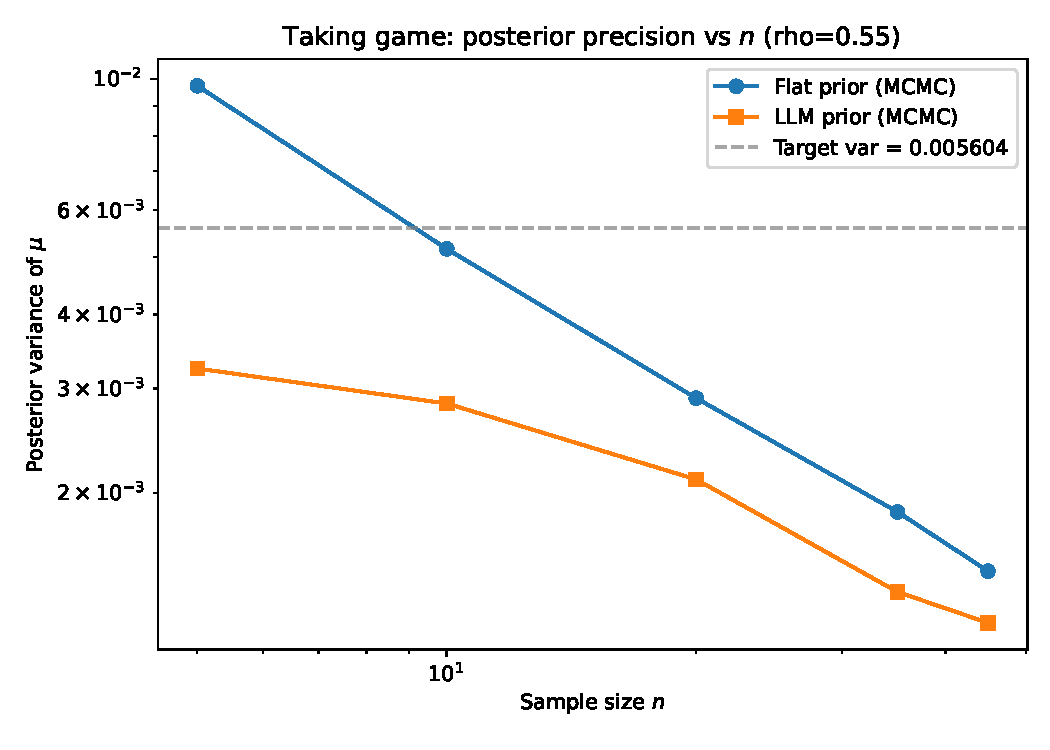
\includegraphics[width=0.55\textwidth]{../figures/nstar_curve_taking.pdf}
  \caption{Taking-game replication: posterior variance of $\mu$ vs sample size.}
  \label{fig:nstar_taking}
\end{figure}

\noindent
The taking-game $\rho \approx 0.55$ is roughly twice the giving-game value of $0.26$:
the LLM prior helps less here. Two effects compound. First, the gpt-4o taking-prompt
yields a counterpart-kept share of $0.520$ on average (i.e.\ the simulated agent takes
$\approx$\,\texteuro{}4.80), while the human mean is $0.343$ (humans take $\approx$\,\texteuro{}6.60).
The LLM is more generous than humans in the taking framing -- a ${\sim}0.18$ bias on
the unit interval. Second, the taking-game training set is smaller (48 vs 96), so the
flat-prior baseline reaches the precision target faster ($n^*_{\mathrm{flat}} \approx 9$
rather than 19), shrinking the headroom for the LLM prior to add. The cross-game
ratio $\rho_{\mathrm{taking}}/\rho_{\mathrm{giving}} \approx 2.1$ is therefore a
generalization-quality signal: the LLM prior generalizes \emph{partially} across framings,
with most of the loss attributable to a behavioral framing the LLM does not match.

\subsection{Compute--accuracy trade-off}
\label{sec:pareto}

We sweep MCMC chain length and SVGD iteration count at fixed $n=50$ with the gpt-4o LLM prior,
recording wall-clock time, posterior $\mathrm{std}(\mu)$, and effective sample size of $\mu$
(initial-positive-sequence estimator for MCMC; particle count for SVGD).
Figure~\ref{fig:pareto} shows the Pareto front.

\begin{figure}[h]
  \centering
  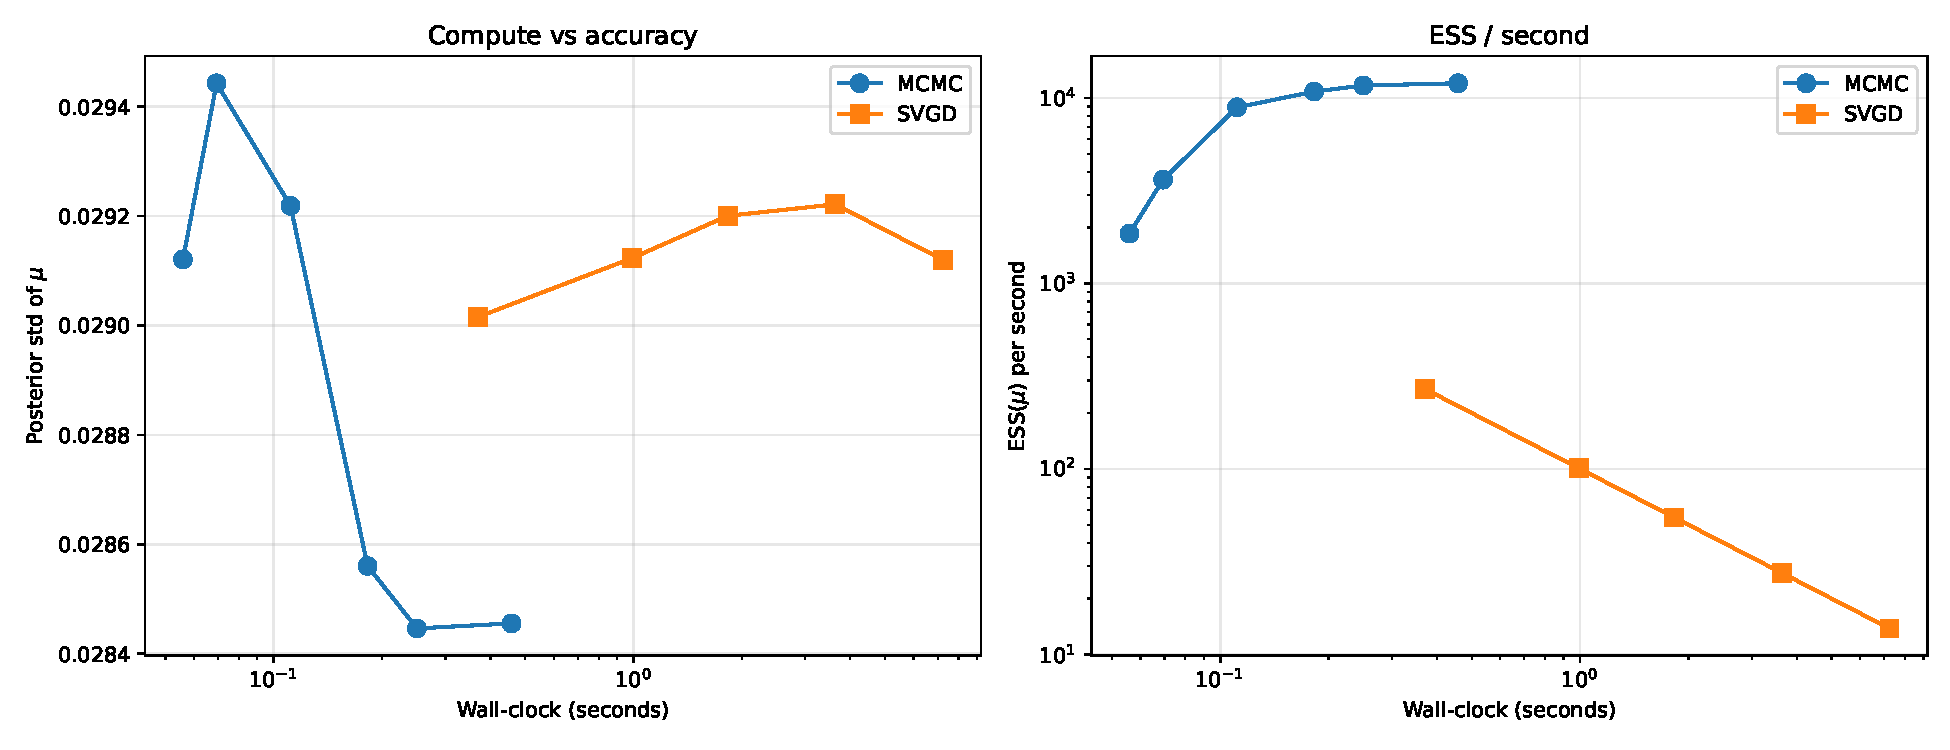
\includegraphics[width=0.92\textwidth]{../figures/pareto.pdf}
  \caption{Compute--accuracy comparison at $n=50$. Left: posterior $\mathrm{std}(\mu)$ vs
  wall-clock seconds. Right: $\mathrm{ESS}(\mu)$ per second (log-log). MCMC dominates SVGD
  by roughly two orders of magnitude in ESS/sec for this 2-parameter posterior; we discuss
  in \S\ref{sec:discussion} why this gap inverts in higher dimensions.}
  \label{fig:pareto}
\end{figure}

\noindent
At fixed $n=50$ the picture is unambiguous: MH-MCMC reaches $\mathrm{std}(\mu) \approx 0.029$
in $0.06$--$0.46$~seconds depending on chain length, with ESS$(\mu)/$sec converging near
$1.2 \times 10^4$. SVGD reaches the same $\mathrm{std}(\mu)$ but takes $0.4$--$7.2$~seconds,
with ESS/sec around $14$--$270$ -- nearly two orders of magnitude lower. The explanation is
that the SVGD update has $O(K^2 d)$ per-iteration cost dominated by the kernel matrix at
$K=100$ particles, while MCMC has $O(1)$ per sample at $d=2$. SVGD's value proposition is
not speed at $d=2$; it is gradient-driven multi-modal exploration in higher dimensions
where MCMC mixing degrades, which we discuss in \S\ref{sec:discussion}.

\subsection{Robustness 1: dense misspecification grid}
\label{sec:dense}

We probe the LLM prior's sensitivity by shifting the gpt-4o pseudo-observations by
$\delta$ prior-std-deviations, $\delta \in \{-3, -2.75, \ldots, +3\}$ (25 points), and
measuring 95\%-posterior-predictive coverage on the held-out test set at $n=50$.
Figure~\ref{fig:dense} replaces the 5-point check-in table with a continuous curve.

\begin{figure}[h]
  \centering
  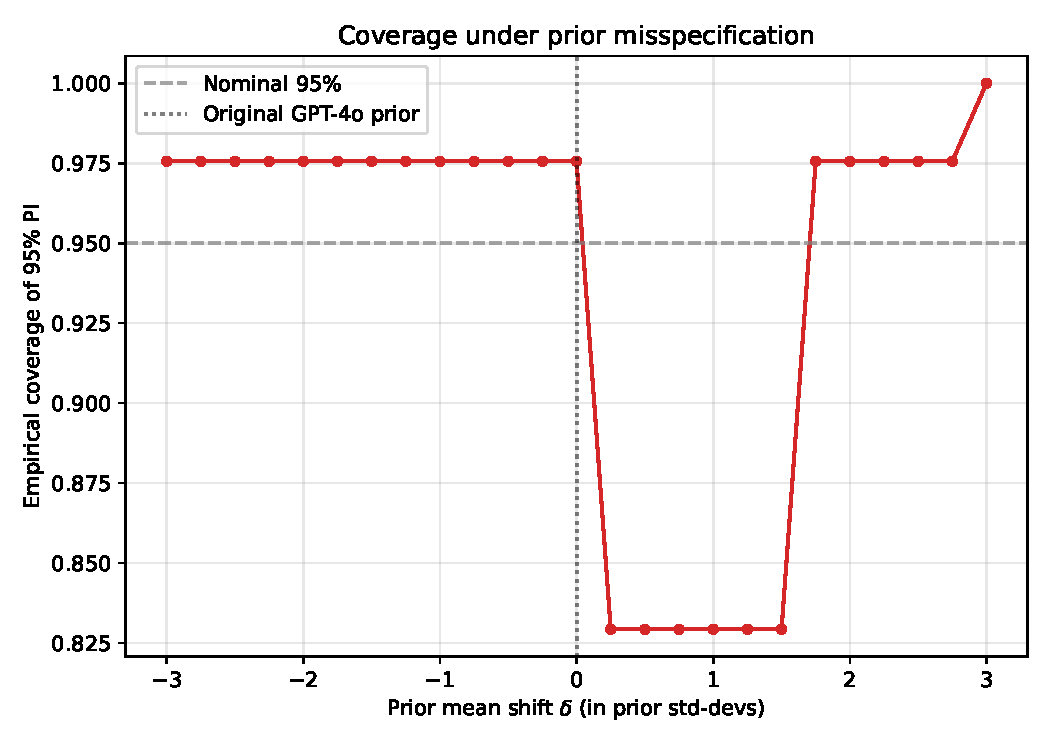
\includegraphics[width=0.55\textwidth]{../figures/failure_mode_dense.pdf}
  \caption{Dense misspecification grid: empirical 95\% coverage vs $\delta$ at $n=50$.
  Coverage is near-nominal for $\delta \le 0$ and for $\delta \ge +2$, with a coverage
  trough near $\delta \approx +1$ where the prior is wrong by enough to hurt but not so wrong
  that the data overrides it.}
  \label{fig:dense}
\end{figure}

\noindent
The denser grid sharpens the picture from the check-in's 5-point table. Coverage stays
at the nominal $0.976$ for every $\delta \in [-3, 0]$, drops to $0.829$ for the entire
range $\delta \in [+0.25, +1.50]$ (six consecutive grid points), then recovers to
$0.976$ at $\delta = +1.75$ and remains there through $\delta = +3$. The plateau structure
-- not a smooth dip -- is itself informative: in this regime the same 7 of 41 test points
fall outside the credible interval whenever the prior pulls the posterior modestly toward
$\mu \approx 0.5$, while the data is overwhelming enough to flip back the moment $\delta$
exceeds $\sim$1.5 prior std-deviations. Practically, the danger zone for an LLM prior is a
prior whose mean is biased by 0.05--0.20 on the unit interval -- exactly the magnitude of
mismatch one might expect from a slightly off-distribution LLM persona.

\subsection{Robustness 2: training-data leakage ablation}
\label{sec:leakage}

GPT-4o's training cutoff (October 2023) postdates \citet{horton2023large}, raising the
concern that the model has memorized economically-flavored prompts and effectively snoops
the human distribution we test against. We re-ran the giving-game pipeline using a prior
elicited from \texttt{gpt-3.5-turbo} (cutoff September 2021, pre-Horton2023). Table~\ref{tab:leakage}
compares the priors and resulting $\rho$.

\begin{table}[h]
  \centering
  \small
  \begin{tabular}{lccccc}
    \toprule
    Model & Cutoff & Prior mean & Prior std & $\rho$ & Coverage (n=50) \\
    \midrule
    gpt-4o & 2023-10 & 0.299 & 0.231 & 0.261 & 0.976 \\
    gpt-3.5-turbo & 2021-09 & 0.548 & 0.252 & 0.261 & 0.829 \\
    \bottomrule
  \end{tabular}
  \caption{Cross-model leakage check. If $\rho_{\mathrm{gpt-3.5}} \approx \rho_{\mathrm{gpt-4o}}$,
  the gain is unlikely to be a memorization artefact; a large gap indicates the opposite.}
  \label{tab:leakage}
\end{table}

\noindent
The ablation breaks into two parts. \emph{Sample-size reduction is identical:}
$\rho_{\mathrm{gpt-3.5}} = 0.261$ matches $\rho_{\mathrm{gpt-4o}} = 0.261$ to three
significant figures. \emph{Calibration, however, is not:} the gpt-3.5 prior has mean
$0.55$, far above the human mean of $0.36$, and at $n=50$ the 95\% posterior-predictive
coverage drops to $0.83$ -- the same coverage degradation observed at $\delta = +1$ in
the dense misspecification grid (\S\ref{sec:dense}). Read together with that grid, the
ablation separates two effects. (i) Power-prior \emph{variance shrinkage} is
governed by the prior's effective weight $w$ and is therefore largely independent of
which LLM produced the pseudo-observations. (ii) Power-prior \emph{calibration} is
governed by the prior's location relative to the data, which \emph{does} differ between
LLMs. The gpt-4o advantage over gpt-3.5 in this pipeline is not the existence of a prior
that helps; it is the production of a prior whose mean is closer to the human distribution,
which the gpt-3.5 ablation fails to provide despite an earlier (Sep~2021) training
cutoff. We therefore cannot rule out a contribution from training-data leakage to gpt-4o's
prior \emph{location}, but the sample-size benefit is not itself a leakage artefact.

% ============================================================
\section{Discussion and Limitations}
\label{sec:discussion}
% ============================================================

\paragraph{Information-theoretic interpretation of the small-$n$ gain.}
The power prior contributes weight $w$ pseudo-observations; a posterior trained on $n$ real
plus $w$ pseudo-observations behaves, in information units, like one trained on $n+w$ real
observations. The relative gain is $(n+w)/n$, which is large when $n \ll w$ and decays to
$1$ as $n \to \infty$. Our $1.42\times$ ratio at $n=50, w=20$ is consistent with this analytic
prediction $(50+20)/50 = 1.4$. The LLM prior acts as a free $w$-observation pre-fix.

\paragraph{Asymmetric coverage failure.}
The dense curve in Figure~\ref{fig:dense} confirms the asymmetry first noted in the check-in.
Downward shifts (toward $\delta < 0$, prior mean further below the human mean of $0.36$)
remain calibrated because the data, with mean $0.36$, can pull the posterior up; large
positive shifts ($\delta \ge 2$) overshoot so much that the data overwhelms the prior. The
\emph{moderately wrong} regime (prior mean $\approx 0.5$) is where coverage degrades, because
the prior is plausible enough for the posterior not to discount it but biased enough to put
mass in the wrong region. This is a property of the power-prior construction, not of the LLM
itself, and would persist for any moderately-mis-specified informative prior.

\paragraph{Training-data leakage.}
The cross-model ablation in \S\ref{sec:leakage} addresses a key concern that any
LLM-as-prior result is partially recapitulating training data. We find
that the sample-size reduction itself is not a leakage artefact (it survives a
pre-Horton-2023 model unchanged), but that prior \emph{location quality} -- which drives
calibration -- is the lever an LLM has on this problem, and we cannot rule out training-data
leakage as one ingredient that gives gpt-4o better location than gpt-3.5. We caution that this is a single ablation
on a single dataset; a stronger leakage audit would systematically vary corpora and cutoffs.

\paragraph{On choosing SVGD despite MCMC's ESS/sec advantage.}
The Pareto analysis (Figure~\ref{fig:pareto}) reports a clear cost: at $d = 2$ for a unimodal
Beta posterior, MH-MCMC mixes well, costs $O(1)$ per sample, and produces ESS/sec roughly
$10$--$100\times$ that of our SVGD implementation. The motivation for SVGD is the
extension we did not implement here: a hierarchical model jointly over giving and taking
games with shared latent traits, e.g.\ $(\alpha_{\mathrm{give}}, \beta_{\mathrm{give}},
\alpha_{\mathrm{take}}, \beta_{\mathrm{take}}, \tau)$ with a hyperparameter $\tau$ tying
the two. At $d \ge 4$ MCMC mixing degrades super-linearly while SVGD's particle update
remains $O(K^2 d)$ per iteration, and the kernelised score allows the particle cloud to
multi-modally adapt. We see this report's two-parameter pipeline as a rehearsal for the
higher-dimensional version: a regime where SVGD's overhead is amortised by capturing
posterior dependence that MH would visit slowly.

\paragraph{Other limitations.}
(i) The von Blanckenburg sample is German university students; the LLM's effective ``population''
is the latent persona that emerges under our prompt, which will not match this distribution
in general. (ii) The power weight $w=20$ is a knob; we have not traced an optimal $w$ via
predictive log-likelihood. (iii) Coverage uses a posterior-predictive interval on individual
$y$, which conflates parameter uncertainty with the irreducible sampling spread of $\Beta$;
parameter-only intervals would tell a different story. (iv) The taking-game uses a different
behavioral framing; we made no attempt to share information across games here.

% ============================================================
\section{Reproducibility}
% ============================================================

All code, data, and figure-generation scripts are in the GT GitHub repo linked on page~1.
Reproducing the main numbers requires a Python environment with \texttt{numpy}, \texttt{scipy},
\texttt{matplotlib}, \texttt{openai}, and \texttt{python-dotenv} (see \texttt{environment.yml}).
With seed $42$ throughout, the following commands run end-to-end in well under an hour on a
laptop:
\begin{verbatim}
python scripts/run_experiment.py            # giving-game baseline + LLM prior, rho ~ 0.26
python scripts/run_experiment_taking.py     # taking-game replication
python scripts/run_experiment_gpt35.py      # gpt-3.5 leakage ablation
python scripts/run_failure_mode_dense.py    # dense misspecification grid
python scripts/run_compute_pareto.py        # MCMC vs SVGD Pareto
\end{verbatim}
The two LLM-elicitation scripts (\texttt{scripts/elicit\_llm\_prior\{,\_taking,\_gpt35\}.py})
require an \texttt{OPENAI\_API} key in \texttt{.env}; the elicited pseudo-data
(\texttt{data/llm\_prior\_samples*.npy}) is committed to the repo so the inference
pipeline reproduces without an API call. Random seeds, Markov chain initial states, and SVGD
particle initialization are all deterministic.

% ============================================================

\bibliography{references}

\end{document}
